%%%%%%%%%%%%%%%%%%%%%%%%%%%%%%%%%%%%%%%%%%%%%%%%%%%
%% LaTeX book template                           %%
%% Author:  Amber Jain (http://amberj.devio.us/) %%
%% License: ISC license                          %%
%%%%%%%%%%%%%%%%%%%%%%%%%%%%%%%%%%%%%%%%%%%%%%%%%%%

\documentclass[a4paper,11pt]{book}
\usepackage[T1]{fontenc}
\usepackage[utf8]{inputenc}
\usepackage{lmodern}
%%%%%%%%%%%%%%%%%%%%%%%%%%%%%%%%%%%%%%%%%%%%%%%%%%%%%%%%%
% Source: http://en.wikibooks.org/wiki/LaTeX/Hyperlinks %
%%%%%%%%%%%%%%%%%%%%%%%%%%%%%%%%%%%%%%%%%%%%%%%%%%%%%%%%%
\usepackage{hyperref}
\usepackage{graphicx}
\usepackage[english]{babel}
\usepackage{amsmath}
\usepackage{amsfonts}
\usepackage{amsthm}
\usepackage{mathtools}

\renewcommand{\vec}[1]{\mathbf{#1}} % Bold Vector Notation
\newcommand{\norm}[1]{\left\lVert#1\right\rVert} % Norm of a Vector
\newcommand{\uvec}[1]{\boldsymbol{\hat{\textbf{#1}}}} % Unit Vector
\newcommand{\Real}{\mathbb{R}}
\newcommand{\Natural}{\mathbb{N}}
\newcommand{\Zahlen}{\mathbb{Z}}
\newcommand{\Quoziente}{\mathbb{Q}}
\newcommand{\newpara}{\\ \newline}


\newtheorem{Theorem}{Theorem}[section]%Theorem
\newtheorem*{Corollary}{Corollary} %Corollary
\newtheorem*{Lemma}{Lemma}%Lemma
\newtheorem*{Statement}{Statement} % Statement
\theoremstyle{definition}
\newtheorem*{Definition}{Definition} %Definition
\newtheorem*{Proposition}{Proposition}%Proposition

%%%%%%%%%%%%%%%%%%%%%%%%%%%%%%%%%%%%%%%%%%%%%%%%
% Chapter quote at the start of chapter        %
% Source: http://tex.stackexchange.com/a/53380 %
%%%%%%%%%%%%%%%%%%%%%%%%%%%%%%%%%%%%%%%%%%%%%%%%
\makeatletter
\renewcommand{\@chapapp}{}% Not necessary...
\newenvironment{chapquote}[2][2em]
  {\setlength{\@tempdima}{#1}%
   \def\chapquote@author{#2}%
   \parshape 1 \@tempdima \dimexpr\textwidth-2\@tempdima\relax%
   \itshape}
  {\par\normalfont\hfill--\ \chapquote@author\hspace*{\@tempdima}\par\bigskip}
\makeatother

%%%%%%%%%%%%%%%%%%%%%%%%%%%%%%%%%%%%%%%%%%%%%%%%%%%
% First page of book which contains 'stuff' like: %
%  - Book title, subtitle                         %
%  - Book author name                             %
%%%%%%%%%%%%%%%%%%%%%%%%%%%%%%%%%%%%%%%%%%%%%%%%%%%

% Book's title and subtitle
\title{\Huge \textbf{Multivariable Calculus}}
% Author
\author{\textsc{Hechen Hu}}


\begin{document}

\frontmatter
\maketitle

%%%%%%%%%%%%%%%%%%%%%%%%%%%%%%%%%%%%%%%%%%%%%%%%%%%%%%%%%%%%%%%%%%%%%%%%
% Auto-generated table of contents, list of figures and list of tables %
%%%%%%%%%%%%%%%%%%%%%%%%%%%%%%%%%%%%%%%%%%%%%%%%%%%%%%%%%%%%%%%%%%%%%%%%
\tableofcontents

\mainmatter

%%%%%%%%%%%%%%%%
% NEW CHAPTER! %
%%%%%%%%%%%%%%%%
\chapter{Vectors in $\mathbb{R} ^n$ Space}

\section{Definition and Properties}
Vector is a geometrical object that has both magnitude and direction. Examples include force and velocity.  \\ Properties in in $n$th dimension vector space for Euclidean vector where $e_i$ is the basis vector for the $i$th axis(for convenience we will us $\vec{i}$, $\vec{j}$, $\vec{k}$ denote the basis vector in a 3-d space):

\section{Addition/Subtraction}

\begin{equation}
\vec{a} \pm \vec{b} = \sum_{i = 1}^{n}(a_i \pm b_i)e_i
\end{equation}

\section{Scalar Multiplication}
\begin{equation}
	k\vec{a} = \sum_{i = 1}^{n}ka_i.e._i
\end{equation}

\section{Dot Product}
\begin{align}
\vec{a} \cdot \vec{b} = &\sum_{i = 1}^{n}a_i * b_i \nonumber \\
								= &\norm{\vec{a}}\norm{\vec{b}}\cos \theta
\end{align}(\textbf{Result is a scalar})
Dot product has the following properties:
\begin{align}
	&(a) \quad \vec{a} \cdot \vec{b} = \vec{b} \cdot \vec{a} \quad (Commutative) \nonumber \\
	&(b) \quad \vec{a} \cdot (\vec{b}+\vec{c}) = \vec{a} \cdot \vec{b} + \vec{a} \cdot \vec{c} \quad (Distributive)\nonumber \\
	&(c) \quad k(\vec{a} \cdot \vec{b}) = (k\vec{a})\cdot\vec{b} = \vec{a} \cdot (k\vec{b}) \quad (Associative) \nonumber \\
	&(d) \quad \vec{a} \cdot \vec{a} = \norm{\vec{a}}^2 \nonumber \\
	&(e) \quad \vec{0} \cdot \vec{a} = 0 \nonumber
\end{align}

\section{Direction Angles\textbackslash Cosines}
The directional angles $\alpha$, $\beta$ and $\gamma$ between the vector $\vec{v}$ and basis vectors $\vec{i}$, $\vec{j}$, $\vec{k}$ in a 3-d space satisfy the following equations:
\begin{align}
&\cos \alpha =  \frac{\vec{v} \cdot \vec{i}} {\norm{\vec{v}} \norm{\vec{i}}} = \frac{v_1}{\norm{\vec{v}}} \\
&\cos \beta =  \frac{\vec{v} \cdot \vec{j}} {\norm{\vec{v}} \norm{\vec{j}}} = \frac{v_2}{\norm{\vec{v}}} \\
&\cos \gamma =  \frac{\vec{v} \cdot \vec{k}} {\norm{\vec{v}} \norm{\vec{k}}} = \frac{v_3}{\norm{\vec{v}}}
\end{align}
According to their definitions we can also see that: \\
\begin{align}
	\cos^2 \alpha + \cos^2 \beta + \cos^2 \gamma &= \frac{{v_1}^2+{v_1}^2 +{v_1}^2}{{\sqrt{{v_1}^2+{v_1}^2 \nonumber +{v_1}^2}}^2} \\
	&= 1
\end{align}

\section{Orthogonal Projections}
The orthogonal projection of $\vec{v}$ on an arbitrary non-zero vector $\vec{b}$ can be written as:
\begin{equation}
	proj_{\vec{b}}\vec{v} = \frac{\vec{v} \cdot \vec{b}}{\norm{\vec{b}}^2}\vec{b}
\end{equation}
Moreover, we can see that $\vec{v} - proj_{\vec{b}}\vec{v}$ is the vector component of $\vec{v}$ orthogonal to $\vec{b}$.


\section{Cross Product}
\begin{align}
\vec{a} \times \vec{b} = 
&\space det \begin{bmatrix}
\vec{i} &\vec{j} &\vec{k} \\
a_1 &a_2 &a_3 \\
b_1 &b_2 &b_3 
\end{bmatrix} \nonumber \\ 
&= (a_2b_3-a_3b_2)\vec{i} - (a_1b_3-a_3b_1)\vec{j} +(a_1b_2-a_2b_1)\vec{k} \nonumber \\ 
&= \norm{\vec{a}}\norm{\vec{b}}\sin \theta \vec{n}
\end{align}
($\vec{n}$ is the vector that perpendicular to both $\vec{a}$ and $\vec{b}$ and its direction is decided by the right hand rule in a right-handed coordinate system.) \\ (Result is a vector that is orthogonal to both $\vec{a}$ and $\vec{b}$) \\

At the same time, we can see that
\begin{align}
&\vec{i} \times \vec{j} = \vec{k} \quad \vec{j} \times \vec{i} = - \vec{k} \\
&\vec{j} \times \vec{k} = \vec{i} \quad \vec{k} \times \vec{j} = - \vec{i} \\
&\vec{k} \times \vec{i} = \vec{j} \quad \vec{i} \times \vec{k} = - \vec{j} 
\end{align}
What's more, the area \boldmath{A} of the parallelogram that has $\vec{a}$ and $\vec{b}$ as adjacent sides is:
\begin{equation}
A = \norm{\vec{a} \times \vec{b}}
\end{equation}
Thus, $\vec{a} \times \vec{b} = 0$ if $\vec{a}$ and $\vec{b}$ are parallel vectors.
More useful properties of cross product:
\begin{align}
&(a) \quad \vec{a} \times \vec{b} = - \vec{b} \times \vec{a} \quad (Anti-Commutative) \nonumber \\
&(b) \quad \vec{a} \times (\vec{b}+\vec{c}) = \vec{a} \times \vec{b} + \vec{a} \times \vec{c} \quad (Distributive)\nonumber \\
&(c) \quad (\vec{b}+\vec{c}) \times \vec{a}  = \vec{b} \times \vec{a} + \vec{c} \times \vec{a} \quad \nonumber \\
&(d) \quad k(\vec{a} \times \vec{b}) = (k\vec{a}) \times \vec{b} = \vec{a} \times (k\vec{b}) \quad (Associative) \nonumber \\
&(e) \quad \vec{a} \times \vec{0} = \vec{0} \times \vec{a} = \vec{0}  \nonumber \\
&(f) \quad \vec{a} \cdot \vec{a} = \vec{0} \nonumber
\end{align}

\section{Scalar triple product}
\begin{align}
(\vec{a} \cdot \vec{b} \times \vec{c}) = det \begin{bmatrix}
a_1 &a_2 &a_3 \\
b_1 &b_2 &b_3 \\
c_1 &c_2 &c_3 
\end{bmatrix}
\end{align}
\textbf{If we switch two rows of this matrix, the product will be multiplied by $-1$.} \\
The absolute value of scalar triple product will give us the volume of the parallelepiped that has $\vec{a}$, $\vec{b}$, $\vec{c}$ as adjacent edges. Therefore, $\vec{a} \cdot (\vec{b} \times \vec{c}) = $ 0 iff they lie on the same plane.

\chapter{Lines and Planes}

\section{Equations of Lines}
The line in 3-d space that passes through the point $P_0(x_0,y_0,z_0)$ and is parallel to the non-zero vector $\vec{v} = <a,b,c> = a\vec{i}+b\vec{j}+c\vec{k}$ has equations:
\begin{align}
	&x = x_0 + at, \quad y = y_0 + bt, \quad z = z_0 + ct \quad(Parametric)\\
	&l = <x_0, y_0, z_0>+t<a,b,c> \quad(Vector)
\end{align}
If two lines doesn't intercept or parallel to each other in a 3-d space, they are skew.

\section{Equations of Planes}
Definition: A vector perpendicular to a plane is called a $\mathbf{normal}$ to that plane. \\
A plane which passing through $P_0(x_0,y_0,z_0)$ and having $\vec{n} = <a,b,c>$as its normal has equations:
\begin{align}
	&a(x-x_0)+b(y-y_0)+c(z-z_0) = 0 \quad (Point-Normal form) \\
	&ax+by+cz+d = 0 \quad (d=-ax_0-by_0-cz_0)(General form)
\end{align}

\section{Angle between Planes}
For two planes that have $\vec{n_1}$ and $\vec{n_2}$ as its normal, the acute angle between them $\theta$ can be obtained from the following equation:
\begin{equation}
	\cos\theta = \frac{|\vec{n_1}\cdot \vec{n_2}|}{\norm{\vec{n_1}}\norm{\vec{n_2}}}
\end{equation}

\section{Distance}
The distance $D$ between a point $P_0(x_0,y_0,z_0)$ and the plane $ax+by+cz+d = 0$ is:
\begin{equation}
	D = \frac{|ax_0+by_0+cz_0+d|}{\sqrt{a^2+b^2+c^2}}
\end{equation}

\textbf{Example: Distance between two skew lines:} \newpara
\textbf{Solution} Find two parallel planes passing through the two skew lines by taking the cross product of their direction vectors, and find the distance between these two planes.\newpara
\\
\textbf{Example: Find the equation of the plane that passes through the line of intersection of the planes $P_1: x-z=1 $ and $ P_2:y+2z=3 $ and is perpendicular to the plane $ P_3:x+y-2z=1 $}.\newpara
\textbf{Solutions:} Find the direction vector for the line of intersection of $ P_1 $ and $ P_2 $ by taking the cross product of their normal vectors. Then take the cross product of the direction vector of the line and the normal vector of $ P_3 $ to find the normal vector of the desired plane. Then find a point on the line of intersection and solve for the plane.

\section{Cylindrical and Spherical Coordinates}
\begin{Definition}
	The three coordinates $ (r, \theta, z) $ of a point $ P $ are defined as:\\
	$ r $ is the Euclidean distance from the $ z $-axis to the point $ P $.\\
	$ \theta $ is the angle between $ x $-axis and the line from the origin to the projection of $ P $ on $ xy $-plane.\\
	The height $ z $ is the signed distance from the $ xy $-plane to the point $ P $.
\end{Definition}
\textbf{Conversion between Rectangular and Cylindrical Coordinates:} \newpara
Suppose the rectangular and cylindrical coordinate of the same point is respectively $ (x,y,z) $ and $ (r,\theta,z) $.
\begin{align}
	&\text{Rectangular to Cylindrical} \nonumber\\
	r &= \sqrt{x^2+y^2}\nonumber \\
	\tan \theta & =\frac{y}{x} \nonumber \\
	z &= z \nonumber \\
	&\text{Cylindrical to Rectangular} \nonumber \\
	x &= r \cos \theta \nonumber \\
	y &= r \sin \theta \nonumber \\
	z &= z \nonumber 
\end{align}
Note that $ \theta $ is not always $ \tan^{-1}\frac{y}{x} $. To find the correct $ \theta $, we must know which quadrant of $ xy $-plane the point lies over.

\begin{Definition}
	The spherical coordinates of a point $ P $ are then defined as follows: \\
	The radius $ \rho $ is the Euclidean distance from the origin $ O $ to $ P $.\\
	The azimuth $ \theta $ is the signed angle measured from the azimuth reference direction to the orthogonal projection of the line segment $ OP $ on the $ xy $-plane.\\
	The inclination $ \phi $ is the angle between the $ z $-axis and the line segment $ OP $.
	
\end{Definition}
\textbf{Conversion Between Spherical and Other Two kinds of Coordinates:} \newpara
Suppose the rectangular, cylindrical, and spherical coordinate of the same point is respectively $ (x,y,z) $, $ (r,\theta,z) $, and $ (\rho,\theta, \phi) $.
$ \theta $ in cylindrical coordinate is the same as $ \theta $ in spherical coordinate.
\begin{align}
	&\text{Spherical to Rectangular or Cylindrical} \nonumber\\
	r &= \rho \sin \phi \nonumber \\
	x &= r \cos \theta = \rho \sin \phi \cos \theta \nonumber \\
	y &= r \sin \theta = \rho \sin \phi \sin \theta \nonumber \\
	z &= \rho \cos \phi\nonumber \\
	&\text{Rectangular to Spherical} \nonumber \\
	\rho &= \sqrt{r^2+z^2}=\sqrt{x^2+y^2+z^2}\nonumber \\
	\tan \theta &= \frac{y}{x} \nonumber \\
	\cos \phi & = \frac{z}{\rho} = \frac{z}{\sqrt{x^2+y^2+z^2}}\nonumber
\end{align}


\chapter{Quadric Surfaces}

\section{Traces}
To help graphing a complex surface in a 3-d space, we obtain traces, or the curves(mesh lines) formed by cutting this surface with well-chosen planes. Usually, surfaces are built up from traces in planes that are parallel to the coordinate planes.

\section{Type of Quadric Surfaces}
\begin{table}
	\begin{tabular}{| c | c | c |}
		\hline
		Name &Equation &Figure  \\ \hline
		Ellipsoid&$\frac{x^2}{a^2}+\frac{y^2}{b^2}+\frac{z^2}{c^2}=1$&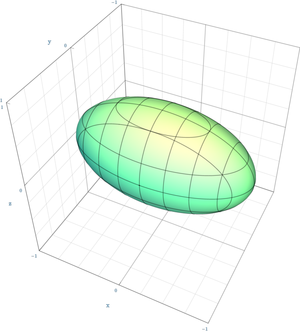
\includegraphics[width=1.1in]{Ellipsoid.png}\\ \hline
		Hyperboloid of one sheet &$\frac{x^2}{a^2}+\frac{y^2}{b^2}-\frac{z^2}{c^2}=1$ &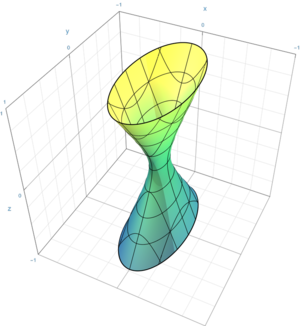
\includegraphics[width=1.5in]{HyperboloidofOneSheet.png} \\ \hline
		Hyperboloid of two sheets &$\frac{z^2}{c^2}-\frac{x^2}{a^2}-\frac{y^2}{b^2}=1$ &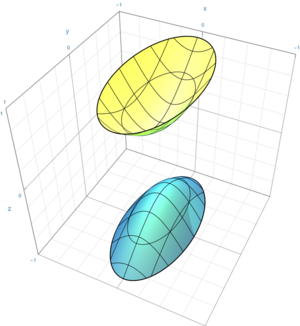
\includegraphics[width=1.5in]{Hyperboloid_Of_Two_Sheets_Quadric.png} \\ \hline
		Elliptic cone &$z^2 = \frac{x^2}{a^2}+\frac{y^2}{b^2}$ &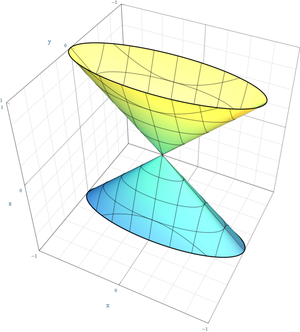
\includegraphics[width=1.2in]{Elliptical_Cone_Quadric.png} \\ \hline
		Elliptic paraboloid &$z = \frac{x^2}{a^2}+\frac{y^2}{b^2}$ &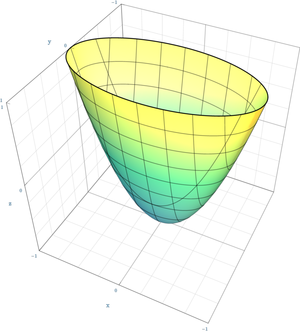
\includegraphics[width=1.5in]{Paraboloid_Quadric.png} \\ \hline
		Hyperbolic paraboloid &$z = \frac{y^2}{b^2}-\frac{x^2}{a^2}$ &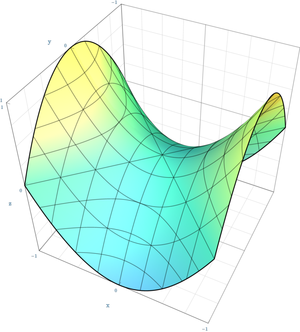
\includegraphics[width=1.5in]{Hyperbolic_Paraboloid_Quadric.png} \\
		\hline
	\end{tabular}
\end{table}

\chapter{Calculus of Vector-Valued Functions}

\section{Orientation/Direction of its graph}
The direction a graph of a vector-valued function goes when its parameter, $t$, increases is called the \textit{orientation} or \textit{direction of increasing parameter}.

\section{Domain and Natural Domain}
The domain of a vector-valued function is the set of all allowable values of $t$.
The natural domain of a vector-valued function is the intersection of its component functions' domain.

\section{Radius Vector/Position Vector}
If a function can be expressed as $F(t) = <f(t),g(t),h(t)>$, then the position vector of it at $t = k$ is $<f(k),g(k),h(k)>$.

\section{Vector Form of A Line Segment}
For two vectors$\vec{r_0}$ and $\vec{r_1}$ that has its initial point at origin, the line passes through the terminal points of them can be written as:
\begin{equation}
	\vec{r} = \vec{r_0} + t(\vec{r_1}-\vec{r_0})
\end{equation}
And this is called the \textbf{\textit{two-point vector form o a line}}.

\section{Calculus of Vector-Valued Functions}
The Calculus of vector-valued functions in 2-d and 3-d space is similar to "normal" functions:\textbf{just apply each operator to its component functions and "sum" them up.} The definition of integrable, differentiable and continuous is also similar:\textbf{each property requires its component functions have the corresponding property.} \\
The tangent line of the graph at point $\vec{r}(t_0)$:
\begin{equation}
	\vec{r}=\vec{t_0}+t\vec{r}^\prime(t_0)
\end{equation}
For the dot product and cross product, which are unique to vector-valued functions, the derivative is defined as following:
\begin{align}
	&\frac{d}{dt}[\vec{r_1}(t) \cdot \vec{r_2}(t)] = \vec{r_1}(t) \cdot \frac{d\vec{r_2}}{dt} +  \frac{d\vec{r_1}}{dt}  \cdot \vec{r_2}(t) \\
	&\frac{d}{dt}[\vec{r_1}(t) \times \vec{r_2}(t)] = \vec{r_1}(t) \times \frac{d\vec{r_2}}{dt} +  \frac{d\vec{r_1}}{dt}  \times \vec{r_2}(t)
\end{align}

In 2-d space, the tangent line to a circle is perpendicular to the radius at the point of tangency. Similarly, in for a vector-valued function, if $\norm{\vec{r}(t)}$ is constant for all $t$, then:
\begin{equation}
	\vec{r}(t)\cdot \vec{r}^\prime(t)=0
\end{equation}
that is, $\vec{r}(t)$ and $\vec{r}^\prime(t)$ are orthogonal for all $t$.

\section{Arc Length}
In a 2-d space, the arc length $L$ of a parametric curve $x=x(t),y=y(t),(a\leq t \leq b)$ can be given as:
\begin{equation}
	L = \int_{a}^{b}{\sqrt{(\frac{dx}{dt})^2+(\frac{dy}{dt})^2}}dt
\end{equation}

\begin{Lemma}
	In a 2-d space, the arc length $L$ of a function $y=f(x)$ that itself and its derivative is continuous on $[a,b]$ is:
	\begin{equation}
		L = \int{ds}
	\end{equation}
	where 
	\begin{align}
		&ds = \sqrt{1+(\frac{dy}{dx})^2}dx \quad if \quad y = f(x), a\leq x \leq b \nonumber \\
		&ds = \sqrt{1+(\frac{dx}{dy})^2}dy \quad if \quad x = g(y), c\leq y \leq d \nonumber
	\end{align}
\end{Lemma}

\begin{proof}
	As we can see in the figure below, the arc length is the sum of distance between $n$ consecutive points when $n\to \infty$ \newline
	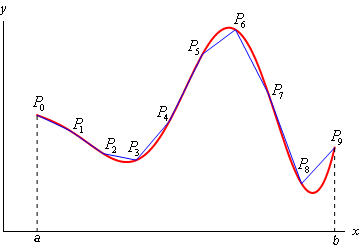
\includegraphics[width=\linewidth]{Curve_Length.png}
	Arc Length $L$ can be written as:
	\begin{equation}
		L = \lim_{n \to \infty}\sum_{i=1}^{n}\sqrt{(x_{i+1}-x_i)^2+(y_{i+1}-y_i)^2} \nonumber \\
	\end{equation}
	Additionally, we can see that
	\begin{equation}
		\sqrt{(x_{i+1}-x_i)^2+(y_{i+1}-y_i)^2} = \sqrt{\Delta x^2+\Delta y_i^2} \nonumber
	\end{equation}
	According to Mean Value Theorem, there exists an $\bar{x}$ such that
	\begin{equation}
		\Delta y_i =  f^\prime(\bar{x_i})\Delta x \nonumber \\
	\end{equation}
	Thus
	\begin{align}
		\sqrt{\Delta x^2+\Delta y_i^2} &= \sqrt{\Delta x^2+\Delta y_i^2} \nonumber \\
												     &= \sqrt{\Delta x^2+(f^\prime(\bar{x_i})\Delta x)^2} \nonumber \\
												     &= \sqrt{1+[f^\prime(\bar{x_i})]^2}\Delta x \nonumber
	\end{align}
	The exact length of the given curve is
	\begin{align}
		L &= \lim_{n \to \infty}\sum_{i=1}^{n}\sqrt{(x_{i+1}-x_i)^2+(y_{i+1}-y_i)^2} \nonumber \\
		   &=  \lim_{n \to \infty}\sum_{i=1}^{n}\sqrt{1+[f^\prime(\bar{x_i})]^2}\Delta x \nonumber \\
		   &= \int_{a}^{b}\sqrt{1+[f^\prime(x)]^2}dx \nonumber \\
		   &= \int_{a}^{b}\sqrt{1+(\frac{dy}{dx})^2}dx \nonumber
	\end{align}
\end{proof}
Now we can prove Theorem (4.6):
\begin{proof}
	Recall that $x = x(t),y = y(t)$, therefore
	\begin{align}
		L &= \int_{a}^{b}\sqrt{1+(\frac{dy}{dx})^2}dx \nonumber \\
		   &= \int_{a}^{b}\sqrt{1+\frac{(\frac{dy}{dt})^2}{(\frac{dx}{dt})^2}}\frac{dx}{dt}dt \nonumber \\
		   &= \int_{a}^{b}\sqrt{1+\frac{(\frac{dy}{dt})^2}{(\frac{dx}{dt})^2}}\frac{dx}{dt}dt \nonumber \\
		   &= \int_{a}^{b}\frac{1}{|\frac{dx}{dt}|}\sqrt{(\frac{dx}{dt})^2+(\frac{dy}{dt})^2}\frac{dx}{dt}dt \nonumber
	\end{align}
	If we assume that $\frac{dx}{dt} \geq 0$,then
	\begin{equation}
		L = \int_{a}^{b}\sqrt{(\frac{dx}{dt})^2+(\frac{dy}{dt})^2}dt \nonumber \\
	\end{equation}
\end{proof}

Analogously, the arc length $L$ of a smoothly parametrized function(\textbf{have a continuously turning tangent vector}) in 3-d space is
\begin{align}
		L &= \int_{a}^{b}\sqrt{(\frac{dx}{dt})^2+(\frac{dy}{dt})^2+(\frac{dz}{dt})^2}dt \nonumber \\
		   &= \int_{a}^{b}\norm{\frac{d\vec{r}}{dt}}dt
\end{align}

\section{Arc Length as A Parameter}
Sometime it would be more convenient to replace $t$ with $s$, which is the length of arc measured along the curve from some fixed reference point. There are three steps: \\
\textbf{Step 1.} Select an reference point.\\
\textbf{Step 2.} Choose one direction from the reference point as the positive direction. \\
\textbf{Step 3.} Change the length $s$ to a "signed" length, which means $s$ is positive if $s$ "moves along the curve" to its positive direction. \\
Note that there are infinitely many different arc length parameterizations. \\
\newline
\begin{Theorem}
	\textbf{Chain Rule} \quad Let $\vec{r}(t)$ be a vector-valued function in 2-d/3-d space that is differentiable with respect to $t$. If $t=g(\tau)$ is a change of parameter in which $g$ is differentiable with respect to $\tau$, then $\vec{r}(g(\tau))$ is differentiable with respect to $\tau$ and
	\begin{equation}
		\frac{d\vec{r}}{d\tau} = \frac{d\vec{r}}{dt}	\frac{dt}{d\tau} 
	\end{equation}
\end{Theorem}
A change in parameter is smooth if $\vec{r}(g(\tau))$ is smooth and $\vec{r}(t)$ is smooth. For all $\tau$,  $\frac{dt}{d\tau}> 0$ is called a positive change of parameter while $\frac{dt}{d\tau}< 0$ is called a negative change of parameter. \\
\newline
\begin{Theorem}
	Let $ C $ be the graph of a smooth vector-valued function $\vec{r}(t)$ in 2-d or 3-d space, and let $\vec{r}(t_0)$ be any point on $ C $. Then the following formula defines a positive change of parameter from $ t $ to $ s $, where $ s $ is an arc length parameter having $\vec{r}(t_0)$ as its reference point:
	\begin{equation}
		s = \int_{t_0}^{t}\norm{\frac{d\vec{r}}{du}}du
	\end{equation}
\end{Theorem} 

\begin{Theorem}
	If $ C $ is the graph of a smooth vector-valued function $\vec{r}(t)$ in 2-d or 3-d space, where $ t $ is a general parameter, and if $ s $ is the arc length parameter for $ C $ defined by \textbf{Theorem 2}, then for every value of $ t $ the tangent vector has length
	\begin{equation}
		\norm{\frac{dr}{dt}}=\frac{ds}{dt}
	\end{equation}
\end{Theorem}
\begin{proof}
	This can be derived from applying the Fundamental Theorem of Calculus to Theorem 2.
\end{proof}

\begin{Theorem}
	If $ C $ is the graph of a smooth vector-valued function $\vec{r}(t)$ in 2-d or 3-d space, where  $ s $ is the arc length parameter, then for every value of $ s $ the tangent vector to $ C $ has length
	\begin{equation}
		\norm{\frac{dr}{ds}}=1
	\end{equation}
\end{Theorem}
\begin{proof}
	Let $ t =s$ in \textbf{Theorem 3}. \nonumber
\end{proof}

\begin{Theorem}
	If $ C $ is the graph of a smooth vector-valued function $ \vec{r}(t) $ in 2-d or 3-d space, and if
	\begin{equation}
		\norm{\frac{dr}{dt}} = 1
	\end{equation}
	for every value of $ t $, then $ t $ is an arc length parameter that has its reference point at the point on $ C $ where $ t=0 $.
\end{Theorem}
\begin{proof}
	The formula
	\begin{equation}
		s = \int_{0}^{t}\norm{\frac{d\vec{r}}{du}}du \nonumber
	\end{equation}
	defines an arc length parameter for $ C $ with reference point $ \vec{r}(0) $. Note that
	\begin{equation}
		\norm{\frac{dr}{dt}} = 1 \nonumber
	\end{equation}
	by hypothesis. Thus the formula can be rewrite as
	\begin{equation}
		s = \int_{0}^{t}du = t - 0 = t \nonumber
	\end{equation}
\end{proof}

\section{Unit Tangent, Normal, and Binormal Vectors}

\begin{Definition}
	The unit tangent of a smooth vector-valued function $ \vec{r}(t) $ in 2-d space or 3-d space that points in the direction of increasing parameter can be expressed as:
	\begin{equation}
		\vec{T}(t)=\frac{\vec{r}^\prime(t)}{\norm{\vec{r}^\prime(t)}}\nonumber
	\end{equation}
	and it's called the \textit{unit tangent vector} to $ C $ at $ t $.
\end{Definition}
Note that for all smooth parameterization which induce the same direction have the same unit tangent vector. \newpara
Recall that if a vector-valued function $ \vec{r}(t) $ has constant norm, then $  \vec{r}(t)  $ and $ \vec{r}^\prime(t) $ are orthogonal. Because $ \vec{T}(t) $ has constant norm $ 1 $, so $ \vec{T}(t) $ and $  \vec{T}^\prime(t) $ are orthogonal. This implies that $ \vec{T}^\prime(t) $ is perpendicular to the tangent line to $ C $ at $ t $, so we say that $ \vec{T}^\prime(t) $ is \textit{normal} to $ C $ at $ t $. If $ \vec{T}^\prime(t) \neq 0 $, then
\begin{equation}
	\vec{N}(t)=\frac{\vec{T}^\prime(t)}{\norm{\vec{T}^\prime(t)}}\nonumber
\end{equation}
is the \textit{principle unit normal vector}, or simply \textit{unit normal vector} to $ C $ at $ t $ and points in the same direction as $ \vec{T}^\prime(t) $. \newpara
The unit normal vector always points toward the concave side of $ C $ in 2-d space. \newpara
According to \textbf{Theorem 4.7.4}, $ \norm{\vec{r}^\prime(t)}=1 $. Thus
\begin{equation}
	\vec{T}(s)=\vec{r}^\prime(s)\nonumber
\end{equation}
and consequently
\begin{equation}
	\vec{N}(s)=\frac{\vec{r}^{\prime\prime}(s)}{\norm{\vec{r}^{\prime\prime}(s)}} \nonumber
\end{equation}

\begin{Definition}
	The binormal vector to $ C $ at $ t $ can be defined as
	\begin{align}
		\vec{B}(t)&=\vec{T}(t)\times\vec{N}(t) \nonumber \\
		&=\frac{\vec{r}^\prime(t)\times\vec{r}^{\prime\prime}(t)}{\norm{\vec{r}^\prime(t)\times\vec{r}^{\prime\prime}(t)}} \nonumber
	\end{align}
	that is, the cross product of its unit tangent vector and unit normal vector and the direction of binormal vector is determined by the right-hand rule. $ \norm{\vec{B}(t)}=1 $ since $ \norm{\vec{T}(t)\times\vec{N}(t)} = \norm{\vec{T}(t)}\norm{\vec{N}(t)}\sin(\pi/2)=1 $. \newpara
	In terms of arc length parameteriation, it can be expressed as 
	\begin{equation}
			\vec{B}(s)=\frac{\vec{r}^\prime(s)\times\vec{r}^{\prime\prime}(s)}{\norm{\vec{r}^{\prime\prime}(s)}} \nonumber
	\end{equation}
\end{Definition}
Together with unit tangent vector and unit normal vector, the binormal vector define three mutually perpendicular planes that point through that point -- the $ \vec{T}\vec{B} $-plane (called the \textit{rectifying plane}), the $ \vec{T}\vec{N} $-plane (called the \textit{osculating plane}), and the $ \vec{N}\vec{B} $-plane (called the \textit{normal plane}). The coordinate system(right-hand) system determined by these three vectors is called the $ \vec{T} \vec{N}\vec{B}$-frame.

\section{Curvature}

\begin{Definition}
	If $ C $ is a smooth curve in 2-d space or 3-d space that is parametrized by arc length, then the \textit{curvature} of $ C $, denoted by $ \kappa = \kappa(s) $, is defined by
	\begin{equation}
		\kappa(s) = \norm{\frac{d\vec{T}}{ds}} = \norm{\vec{r}^{\prime\prime}(s)} \nonumber
	\end{equation}
\end{Definition}

\begin{Theorem}
	If $ \vec{r}(t) $ is a smooth vector-valued function in 2-d space or 3-d space, then for each value of $ t $ at which $ \vec{T}(t) $ and $ \vec{r}^{\prime\prime}(t) $ exist, the curvature $ \kappa $ can be expressed as
	\begin{align}
		\kappa(t)&=\frac{\norm{\vec{T}^\prime(t)}}{\norm{\vec{r}^\prime(t)}} \nonumber\\
		&= \frac{\norm{\vec{r}^\prime(t)\times\vec{r}^{\prime\prime}(t)}}{\norm{\vec{r}^\prime(t)}^3} \nonumber
	\end{align}
\end{Theorem}

\begin{Definition}
	If at $ P $ $ \kappa \neq 0 $, then there exists a unique circle $ \Omega $ passing through $ P $ on the concave side of $ C $ such that the curvature of $ \Omega $ is $ \kappa $ and it shares a common tangent vector with $ C $. Then $ \Omega $ is called a \textit{osculating circle} or \textit{circle of curvature} at $ P $, $ 1/\kappa  $ is called the radius of curvature at $ P $, and the center of $ \Omega $ is called the center of curvature at $ P $.
\end{Definition}

\begin{Definition}
	Let $ \phi(s) $ be the angle measured counterclockwise from the direction of the positive $ x $-axis to the unit tangent vector $ T $ \textbf{in terms of arc length}. Then
	\begin{equation}
		\kappa(s)=|\frac{d\phi}{ds}| \nonumber
	\end{equation}
\end{Definition}

\section{Motion Along A Curve}
\begin{Definition}
	If a particle moves along a smooth vector-valued function $ \vec{r}(t) $, then the velocity of this particle is
	\begin{equation}
		\vec{v}(t)=\vec{r}^\prime(t)=\frac{ds}{dt}\vec{T}(t)\nonumber
	\end{equation}
	where $ \vec{v}(t) $ is the tangent vector at $ t $. The direction of $ \vec{v}(t) $ gives the instantaneous direction of motion at $ t $. The magnitude of $ \vec{v}(t) $ is the instantaneous rate of change of arc length as a function of time, or just simply speed.
\end{Definition}

\begin{Definition}
	The acceleration of this particle with velocity of $ \vec{v}(t) $ is $ \vec{a}(t)=\vec{v}^\prime(t)=\vec{r}^{\prime\prime}(t) $. What's more
	\begin{equation}
		\vec{a}(t)=\frac{d^2s}{dt^2}\vec{T}(t)+\kappa(t)(\frac{ds}{dt})^2\vec{N}(t)\nonumber
	\end{equation}
	If the particle is travelling on a circle with radius $ r $, the speed $ v_0 $ is constant, and $ \norm{\vec{a}(t)}=\frac{v_0^2}{r} $.
\end{Definition}

\begin{Statement}
	Over a time interval $ [t_1,t_2] $, the distance traveled by a particle is
	\begin{equation}
		s=\int_{t_1}^{t_2}\norm{\vec{v}(t)}dt\nonumber
	\end{equation}
\end{Statement}

\begin{Definition}
	If $ a_T= \frac{d^2s}{dt^2}$ and $ a_N= \kappa(t)(\frac{ds}{dt})^2$, then
	\begin{equation}
		\vec{a}=a_T\vec{T}+a_N\vec{N} \nonumber
	\end{equation}
	and $ a_T $ is called the \textit{tangential component of acceleration} and $ a_N $ is called \textit{normal component of acceleration} . $ a_T\vec{T} $ is the \textit{tangential vector component of acceleration} and $ a_N\vec{N} $ is called the \textit{normal vector component of acceleration}
\end{Definition}

\begin{Statement}
	\begin{align}
		a_T&=\frac{\vec{v}\cdot \vec{a}}{\norm{\vec{v}}} \nonumber\\
		a_N&=\frac{\norm{\vec{v}\times \vec{a}}}{\norm{\vec{v}}} \nonumber\\
		\kappa&=\frac{\norm{\vec{v}\times \vec{a}}}{\norm{\vec{v}}^3} \nonumber
	\end{align}
\end{Statement}
In 2-d space, the cross product can be computed by viewing $ \vec{r}(t)=<x(t),y(t)> $ as $ \vec{r}(t)=<x(t),y(t),0> $ in 3-d space.
\begin{Statement}
	\begin{equation}
		\norm{\vec{a}}^2=\vec{a}_T^2+\vec{a}_N^2 \nonumber
	\end{equation}
	for all smooth position functions.
\end{Statement}

\section{Projectile Motion}
\begin{Theorem}
	For a projectile motion
	\begin{align}
		\vec{r}(t)&=-\frac{gt^2}{2}\vec{j}+t\vec{v}_0+s_0\vec{j} \nonumber \\
		&= (-\frac{gt^2}{2}+s_0 )\vec{j}+t\vec{v}_0 \nonumber
	\end{align}
	where $ g $ is the gravitational acceleration, $ v_0 $ is the initial velocity, and $ s_0 $ is the initial height.
	
\end{Theorem}



\chapter{Multivariable Calculus}
\section{Definition of Multivariable functions and their graph}
\begin{Definition}
	A \textit{real-valued function $ f $ of $ n $ real variables} is a mapping that assign an ordered pair of $ n $ real numbers to a real number in $ D\subset \Real^n $.
\end{Definition}

\begin{Definition}
	If $ f $ is a function of two variables and $ k $ is a real number, then the \textit{level curve of $ f $ of height $ k $} is $ \{(x,y)|f(x,y)=k\} $. A collection of many level curves for a function $ f $ all drawn in the same $ xy $-plane is called a \textit{contour plot/map} of $ f $.
\end{Definition}

\section{Properties of Sets in 2-d and 3-d space}
\begin{Definition}
	For $ r>0 $ and a point $ P $, the \textit{open ball of radius $ r $ centered at $ P $} means the set of all points whose distance to $ P $ is less than $ r $ and denotes $ B_r(P) $.
\end{Definition}
Suppose $ D \subset \Real^2 $ or $ D \subset \Real^3 $.
\begin{Definition}
	A point $ P $ is said to be an \textit{interior point} of $ D $ if $ \exists r>0(B_r(P)\subset D) $.
\end{Definition}
\begin{Definition}
	A point $ P $ is said to be an \textit{boundary point} of $ D $ if $ \forall r>0 ((B_r(P) \cap D \neq \emptyset)\land(B_r(P)\setminus D \neq \emptyset)) $
\end{Definition}

\begin{Definition}
	For a set $ D $ in 2-d and 3-d space, the set of all its interior points is called the \textit{interior} of $ D $. The set of all its boundary points is called the \textit{boundary} of $ D $.
\end{Definition}

\begin{Definition}
	A set is to be said \textit{open} if it contains none of its boundary points, and when it contains all of its boundary points, it's called a \textit{closed} set.
\end{Definition}

However, some sets are \textbf{neither} open or close.
\begin{Statement}
	A set $ D $ in $ n $-space is both open and closed iff $ D=\Real^n $ or $ D = \emptyset $.
\end{Statement}

\begin{Definition}
	A subset $ D $ of $ \Real^n $ is said to be \textit{bounded} if $ \exists r>0\exists P(D\subset B_r(P)) $. That is, the set is contained in some set with finite radius. It's \textit{unbounded} if it's not bounded.
\end{Definition}

\begin{Definition}
	A point $ P $ is said to be the \textit{accumulation point} of some $ D \subset \Real^n $ if $ \forall r>0(B_r(P)\setminus D \setminus\{P\}\neq \emptyset) $.
\end{Definition}



\end{document}
